\FloatBarrier
\begin{figure}[!h]
\centering
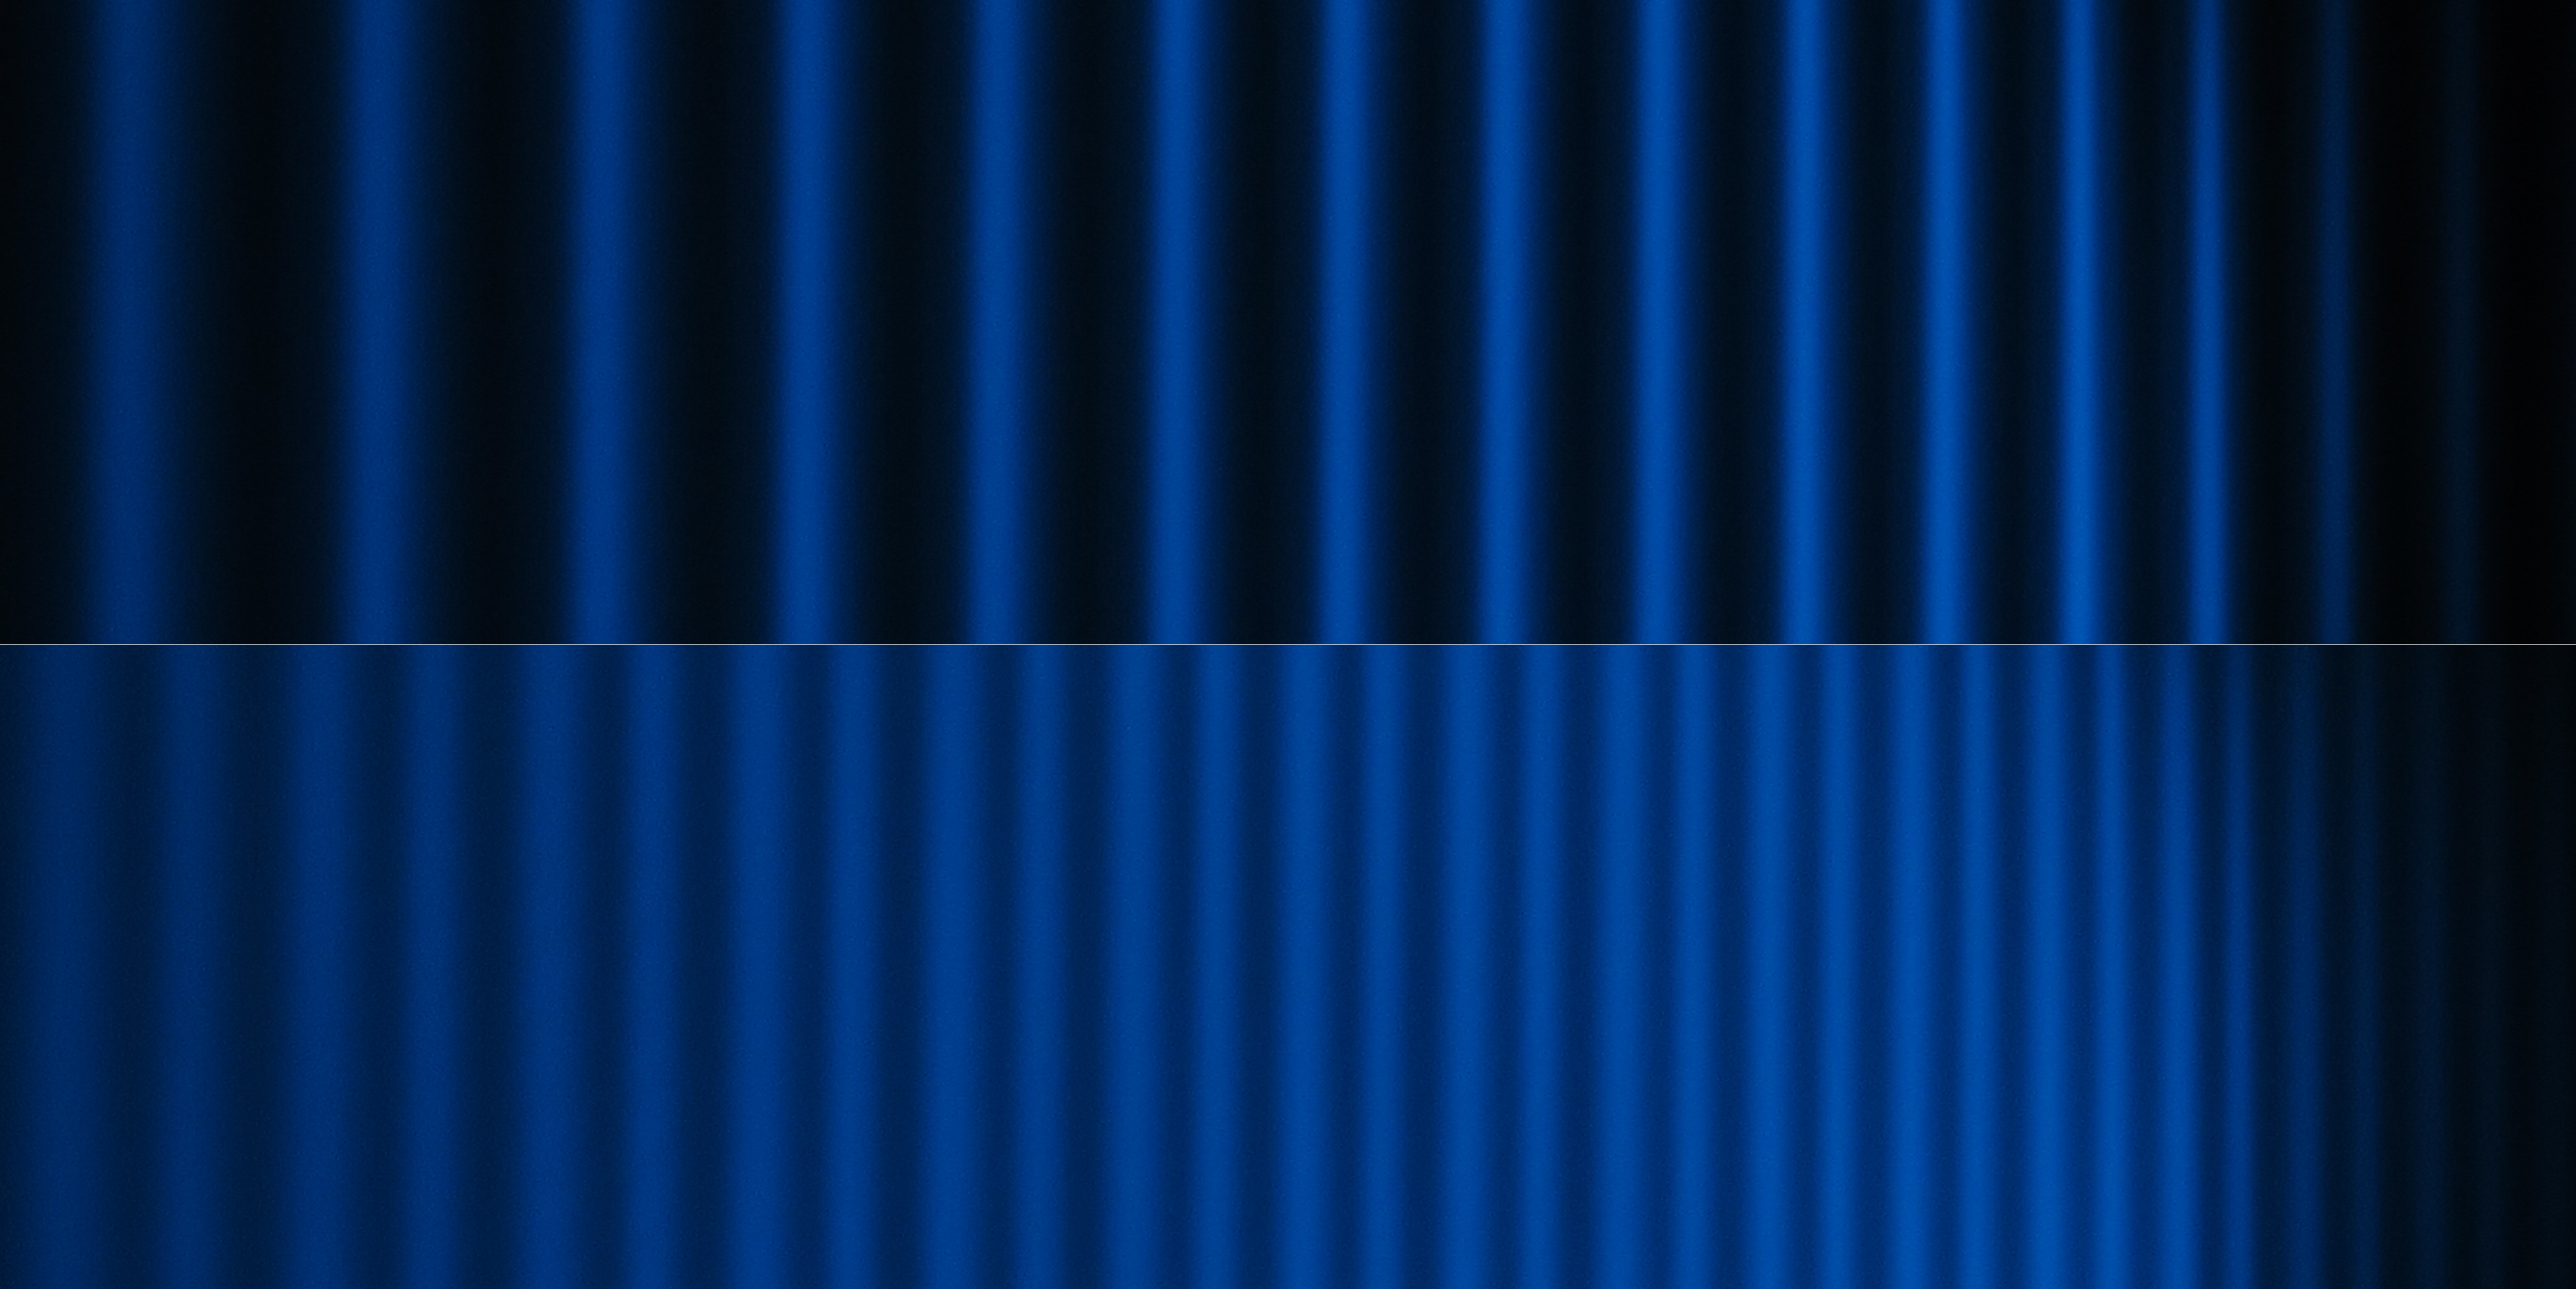
\includegraphics[scale=0.1]{../Grafiken/3-I0_t8_sigma_4-I5_t8_sigma.jpg}
\caption{Aufnahmen der blauen $\sigma$-Spekrallinie. Im oberen Teil ist die
        Spektrallinie ohne Einfluss eines äußeren Magnetfeldes abgebildet.
        Im unteren Teil ist die Zeemann-Aufspaltung der Spektrallinie
        im äußeren Magnetfeld zu erkennen.
        Obwohl diese Spektrallinie in vier $\sigma$-Linien aufspaltet sind nur
        zwei Linien zu erkennen, da sich je zwei der vier Linien überlagern. 
        \label{fig:3-i0_t8_sigma_4-i5_t8_sigma}}
\end{figure}
\FloatBarrier
